\documentclass[10pt,preprint]{../aastex}

\usepackage{amsfonts}
\usepackage{amsmath}
\usepackage{amssymb}
\usepackage{amsthm}
\usepackage{booktabs}
\usepackage{mathrsfs}
\usepackage{cite}
\usepackage{times}
\usepackage{url}
\usepackage{hyperref}
\usepackage{lineno}
\usepackage{yhmath}
\usepackage{natbib}
\usepackage{../../definitions}
\hypersetup{
  bookmarksnumbered = true,
  bookmarksopen=false,
  pdfborder=0 0 0,         % make all links invisible, so the pdf looks good when printed
  pdffitwindow=true,      % window fit to page when opened
  pdfnewwindow=true, % links in new window
  colorlinks=true,           % false: boxed links; true: colored links
  linkcolor=blue,            % color of internal links
  citecolor=magenta,    % color of links to bibliography
  filecolor=magenta,     % color of file links
  urlcolor=cyan              % color of external links
}

\usepackage{float}
\usepackage{graphicx}
\newtheorem{remark}{Remark}
\graphicspath{{Figures/}}
\newcommand{\figref}[1]{Figure \ref{#1}}

\begin{document}

\section{Derivation of Middle Wave-Speed Estimate for General Relativistic HLLC Numerical Flux}
For a given Riemann problem we assume that the shocked fluid is composed of two distinct regions, separated by a contact discontinuity (see \figref{Fig:HLLC_RiemannFan}).
\begin{figure}[H]
\centering
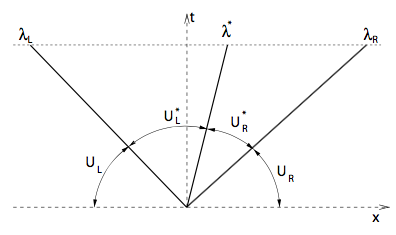
\includegraphics[scale=0.5]{HLLC_RiemannFan_MB2005}
\caption{HLLC Riemann fan from \citet{Mignone2005}.}\label{Fig:HLLC_RiemannFan}
\end{figure}


Here we derive an estimate for the propagation speed of that contact discontinuity.

The equations we are solving are the general relativistic equations of hydrodynamics in conservative form:
\begin{equation}
    \pderiv{\left(\sqrtgm\,\bU\right)}{t}+\pderiv{\left(\alpha\,\sqrtgm\,\bF^{i}\left(\bU\right)\right)}{x^{i}}=\alpha\,\sqrtgm\,\bS,
\end{equation}
where $\bU$ is the \textit{vector of conserved variables}, $\bF^{i}\left(\bU\right)$ are the fluxes of the conserved variables along the three spatial directions, $\bS$ is a source term (which does \textit{not} contain any derivatives of the fluid variables), $\alpha$ is the lapse function, and $\sqrtgm$ is the determinant of the spatial three-metric. In deriving the above equations we assume that the lapse function is explicitly independent of time. We can re-write this slightly using the product rule:
\begin{equation}
    \sqrtgm\,\pderiv{\bU}{t}+\bU\,\pderiv{\sqrtgm}{t}+\sqrtgm\,\pderiv{\left(\alpha\,\bF^{i}\right)}{x^{i}}+\alpha\,\bF^{i}\,\pderiv{\sqrtgm}{x^{i}}=\alpha\,\sqrtgm\,\bS.
\end{equation}
Now, moving the terms that don't contain derivatives of the fluid variables to the RHS and dividing by $\sqrtgm$, we obtain:
\begin{equation}\label{Eq:EulerConsSources}
    \pderiv{\bU}{t}+\pderiv{\left(\alpha\,\bF^{i}\right)}{x^{i}}=\bQ,
\end{equation}
where:
\begin{equation}
    \bQ\equiv\alpha\,\bS-\f{1}{\sqrtgm}\left(\bU\,\pderiv{\sqrtgm}{t}+\alpha\,\bF^{i}\,\pderiv{\sqrtgm}{x^{i}}\right).
\end{equation}

The vector of conserved variables is given by \citep{Mignone2005}:
\begin{equation}
    \bU\equiv
    \begin{pmatrix}
      D \\
      S_{j} \\
      E
    \end{pmatrix}=
    \begin{pmatrix}
      \rho\,W \\
      \rho\,h\,W^{2}\,v_{j} \\
      \rho\,h\,W^{2}-p,
    \end{pmatrix}
\end{equation}
where $\rho$ is the rest mass-density, $v_{j}$ are the covariant components of the three-velocity, $p$ is the pressure, and $W$ is the Lorentz factor:
\begin{equation}
    W\equiv\left(1-\vv{v}\cdot\vv{v}\right)^{-1/2}.
\end{equation}
The quantity $h$ is the relativistic specific enthalpy, given by:
\begin{equation}
    h\equiv1+\f{e+p}{\rho},
\end{equation}
where $e$ is the internal energy-density. The fluxes are given by \citep{RezzollaRelHyd}:
\begin{equation}
    \bF^{i}\equiv
    \begin{pmatrix}
      D\left(v^{i}-\alpha^{-1}\,\beta^{i}\right) \\
      S_{j}\left(v^{i}-\alpha^{-1}\,\beta^{i}\right) + p\,\delta^{i}_{~j} \\
      S^{i}-\alpha^{-1}\,\beta^{i}\,E
    \end{pmatrix},
\end{equation}
where $\beta^{i}$ are the components of the shift vector. We define the quantity $\eta^{i}$ as:
\begin{equation}
    \eta^{i}\equiv\alpha^{-1}\,\beta^{i},
\end{equation}
which makes the fluxes that we work with:
\begin{equation}
    \bF^{i}\equiv
    \begin{pmatrix}
      D\left(v^{i}-\eta^{i}\right) \\
      S_{j}\left(v^{i}-\eta^{i}\right) + p\,\delta^{i}_{~j} \\
      S^{i}-\eta^{i}\,E
    \end{pmatrix}.
\end{equation}

We will need to know how the fluxes relate to the conserved variables across shocks. These relations are known as the \textit{Rankine-Hugoniot jump conditions}. We derive them next.

\subsection{Derivation of Rankine-Hugoniot Jump Conditions}
This derivation closely follows \citet{RezzollaRelHyd}.

We start the derivation by integrating the one-dimensional version of \eqref{Eq:EulerConsSources} in space from a point $x_{L}$ to a point $x_{R}$, that contains a shock, which we define to be at a time-dependent point $x_{L}<s\left(t\right)<x_{R}$:
\begin{equation}
    \int\limits_{x_{L}}^{x_{R}}\pd{\bU}{t}\,\sqrtgm\,dx+\int\limits_{x_{L}}^{x_{R}}\pd{\left(\alpha\,\bF\right)}{x}\,\sqrtgm\,dx=\int\limits_{x_{L}}^{x_{R}}\bQ\,\sqrtgm\,dx.
\end{equation}
Using the product rule again, we get:
\begin{equation}
    \int\limits_{x_{L}}^{x_{R}}\pd{\left(\sqrtgm\,\bU\right)}{t}\,dx-\int\limits_{x_{L}}^{x_{R}}\bU\,\pd{\sqrtgm}{t}\,dx+\int\limits_{x_{L}}^{x_{R}}\pd{\left(\alpha\,\sqrtgm\,\bF\right)}{x}\,dx-\int\limits_{x_{L}}^{x_{R}}\alpha\,\bF\,\pd{\sqrtgm}{x}\,dx=\int\limits_{x_{L}}^{x_{R}}\bQ\,\sqrtgm\,dx.
\end{equation}
Again moving the terms that don't contain derivatives of fluid variables to the RHS, we get:
\begin{equation}
    \int\limits_{x_{L}}^{x_{R}}\pd{\left(\sqrtgm\,\bU\right)}{t}\,dx+\int\limits_{x_{L}}^{x_{R}}\pd{\left(\alpha\,\sqrtgm\,\bF\right)}{x}\,dx=\int\limits_{x_{L}}^{x_{R}}\,\bQ'\,\sqrtgm\,dx,
\end{equation}
where
\begin{equation}
    \bQ'\equiv\bQ+\f{1}{\sqrtgm}\left(\bU\,\pd{\sqrtgm}{t}+\alpha\,\bF\,\pd{\sqrtgm}{x}\right).
\end{equation}

The second term on the LHS becomes a boundary term. Moving that to the RHS and the source term to the LHS we get:
\begin{equation}
    \alpha\left(x_{L},t\right)\,\sqrtgm\left(x_{L},t\right)\,\bF\left(\bU\left(x_{L},t\right)\right)-\alpha\left(x_{R},t\right)\,\sqrtgm\left(x_{R},t\right)\,\bF\left(\bU\left(x_{R},t\right)\right)=\f{d}{dt}\int\limits_{x_{L}}^{x_{R}}\sqrtgm\,\bU\,dx-\int\limits_{x_{L}}^{x_{R}}\bQ'\,\sqrtgm\,dx.
\end{equation}
We now split the first integral into two parts, with the shock being at an endpoint:
\begin{equation}
    \alpha_{L}\,\sqrtgm_{L}\,\bF_{L}-\alpha_{R}\,\sqrtgm_{R}\,\bF_{R}=\f{d}{dt}\int\limits_{x_{L}}^{s_{L}\left(t\right)}\sqrtgm\,\bU\,dx+\f{d}{dt}\int\limits_{s_{R}\left(t\right)}^{x_{R}}\sqrtgm\,\bU\,dx-\int\limits_{x_{L}}^{x_{R}}\sqrtgm\,\bQ'\,dx,
\end{equation}
where $\bF_{L}\equiv\bF\left(\bU\left(x_{L},t\right)\right)$, etc. We also use the notation that $s_{L}$ means ``approaches $s$ from the left state" and $s_{R}$ means ``approaches $s$ from the right state". Using the rule for differentiating an integral with variable bounds:
\begin{equation}
    \f{d}{dt}\int\limits_{x_{1}\left(t\right)}^{x_{2}\left(t\right)}A\left(x,t\right)\,dx=\int\limits_{x_{1}\left(t\right)}^{x_{2}\left(t\right)}\pd{A\left(x,t\right)}{t}\,dx+A\left(x_{2}\left(t\right),t\right)\,\f{dx_{2}\left(t\right)}{dt}-A\left(x_{1}\left(t\right),t\right)\,\f{dx_{1}\left(t\right)}{dt},
\end{equation}
we find:
\begin{equation}
    \alpha_{L}\,\sqrtgm_{L}\,\bF_{L}-\alpha_{R}\,\sqrtgm_{R}\,\bF_{R}=\f{ds}{dt}\left(\sqrtgm_{L}\,\bU_{L}-\sqrtgm_{R}\,\bU_{R}\right)+\int\limits_{x_{L}}^{s_{L}\left(t\right)}\pd{\left(\sqrtgm\,\bU\right)}{t}\,dx+\int\limits_{s_{R}\left(t\right)}^{x_{R}}\pd{\left(\sqrtgm\,\bU\right)}{t}\,dx-\int\limits_{x_{L}}^{x_{R}}\bQ'\,dx.
\end{equation}
Now we take the limit that $x_{L}\longrightarrow s\left(t\right)$ and $x_{R}\longrightarrow s\left(t\right)$. In this limit all the integrals vanish (since no terms in $\bQ'$ depend on derivatives of fluid variables), and since $\alpha$ and $\sqrtgm$ are continuous across shocks, $\alpha_{L}=\alpha_{R}\equiv\alpha$ and $\sqrtgm_{L}=\sqrtgm_{R}\equiv\sqrtgm$. Defining the shock speed as $ds/dt\equiv\lambda$, we see that the metric determinant cancels, leaving us with the jump conditions:
\begin{equation}
    \alpha\left(\bF_{L}-\bF_{R}\right)=\lambda\left(\bU_{L}-\bU_{R}\right).
\end{equation}


\subsection{Derivation of Contact Wave-Speed}
With the jump conditions we are ready to derive an estimate for the propagation speed of the contact discontinuity. If we assume one state is the shocked region and the other state is the unshocked region then the jump conditions become:
\begin{equation}\label{Eq:RHJump_GR}
    \lambda^{i}\left(\bU^{*}-\bU\right)=\alpha\left(\left(\bF^{*}\right)^{i}-\bF^{i}\right).
\end{equation}
We assume that the flux in the shocked region can be written as:
\begin{equation}
    \left(\bF^{*}\right)^{i}\equiv
    \begin{pmatrix}
      D^{*}\left[\left(v^{*}\right)^{i}-\left(\eta^{*}\right)^{i}\right] \\
      S^{*}_{j}\left[\left(v^{*}\right)^{i}-\left(\eta^{*}\right)^{i}\right] + p^{*}\,\delta^{i}_{~j} \\
      \left(S^{*}\right)^{i}-\left(\eta^{*}\right)^{i}\,E^{*}
    \end{pmatrix}.
\end{equation}
Since $\alpha$ and $\boldsymbol{\beta}$ are continuous, we can equate $\alpha^{*}=\alpha$ and $\boldsymbol{\beta}^{*}=\boldsymbol{\beta}$, and therefore $\left(\eta^{*}\right)^{i}=\eta^{i}$. We also define $\left(v^{*}\right)^{i}\equiv\left(\lambda^{*}\right)^{i}$, the propagation speed of the contact discontinuity. We use the shorthand notation:
\begin{equation}
    \left(X^{*}\right)^{i}=X^{*i}.
\end{equation}
With that the fluxes in the shocked region can be written as:
\begin{equation}\label{Eq:StarFlux}
    \bF^{*i}\equiv
    \begin{pmatrix}
      D^{*}\left(\lambda^{*i}-\eta^{i}\right) \\
      S^{*}_{j}\left(\lambda^{*i}-\eta^{i}\right) + p^{*}\,\delta^{i}_{~j} \\
      S^{*i}-\eta^{i}\,E^{*}
    \end{pmatrix}.
\end{equation}

\subsubsection{Applying the Jump Conditions}
Now we apply the jump conditions, \eqref{Eq:RHJump_GR} to the momentum-density:
\begin{align}
    \lambda^{i}\left(S^{*}_{j}-S_{j}\right)&=\alpha\left[S^{*}_{j}\left(\lambda^{*i}-\eta^{i}\right)+p^{*}\,\delta^{i}_{~j}-S_{j}\left(v^{i}-\eta^{i}\right)-p\,\delta^{i}_{~j}\right]\\
    \implies S^{*}_{j}\left(\lambda^{i}-\alpha\,\lambda^{*i}+\alpha\,\eta^{i}\right)&=S_{j}\left(\lambda^{i}-\alpha\,v^{i}+\alpha\,\eta^{i}\right)+\alpha\left(p^{*}-p\right)\delta^{i}_{~j}\label{Eq:RH_Mom}
\end{align}

Before we apply the jump conditions to the energy-density, we note that:
\begin{align}
    S^{i}&=\left(E+p\right)v^{i}\\
    S^{*i}&=\left(E^{*}+p^{*}\right)\lambda^{*i}.\label{Eq:SsEs}
\end{align}
Next we apply the jump conditions to the energy-density:
\begin{align}
    \lambda^{i}\left(E^{*}-E\right)&=\alpha\left(S^{*i}-\eta^{i}\,E^{*}-S^{i}+\eta^{i}\,E\right)\\
    \implies\lambda^{i}\left(E^{*}-E\right)&=\alpha\left(E^{*}\,\lambda^{*i}+p^{*}\,\lambda^{*i}-\eta^{i}\,E^{*}-E\,v^{i}-p\,v^{i}+\eta^{i}\,E\right)\\
    \implies E^{*}\left(\lambda^{i}-\alpha\,\lambda^{*i}+\alpha\,\eta^{i}\right)&=E\left(\lambda^{i}-\alpha\,v^{i}+\alpha\,\eta^{i}\right)+\alpha\left(p^{*}\,\lambda^{*i}-p\,v^{i}\right).\label{Eq:RH_E}
\end{align}
Now we use \eqref{Eq:SsEs} and re-write \eqref{Eq:RH_Mom} (using the metric to raise and lower indices, so $S^{*}_{j}=\gamma_{jk}S^{*k}$):
\begin{equation}
    \left(E^{*}+p^{*}\right)\gamma_{kj}\,\lambda^{*k}\left(\lambda^{i}-\alpha\,\lambda^{*i}+\alpha\,\eta^{i}\right)=S_{j}\left(\lambda^{i}-\alpha\,v^{i}+\alpha\,\eta^{i}\right)+\alpha\left(p^{*}-p\right)\delta^{i}_{~j}.
\end{equation}
Slight manipulation yields:
\begin{equation}
    E^{*}\left(\lambda^{i}-\alpha\,\lambda^{*i}+\alpha\,\eta^{i}\right)=-p^{*}\left(\lambda^{i}-\alpha\,\lambda^{*i}+\alpha\,\eta^{i}\right)+\f{S_{j}\left(\lambda^{i}-\alpha\,v^{i}+\alpha\,\eta^{i}\right)+\alpha\left(p^{*}-p\right)\delta^{i}_{~j}}{\gamma_{kj}\,\lambda^{*k}}.
\end{equation}
Now we equate this with \eqref{Eq:RH_E}, which gives:
\begin{equation}
    E\left(\lambda^{i}-\alpha\,v^{i}+\alpha\,\eta^{i}\right)+\alpha\left(p^{*}\,\lambda^{*i}-p\,v^{i}\right)=-p^{*}\left(\lambda^{i}-\alpha\,\lambda^{*i}+\alpha\,\eta^{i}\right)+\f{S_{j}\left(\lambda^{i}-\alpha\,v^{i}+\alpha\,\eta^{i}\right)+\alpha\left(p^{*}-p\right)\delta^{i}_{~j}}{\gamma_{kj}\,\lambda^{*k}}.
\end{equation}
Or, multiplying through by $\gamma_{kj}\,\lambda^{*k}$:    
\begin{align}
    &\gamma_{kj}\,\lambda^{*k}\left[E\left(\lambda^{i}-\alpha\,v^{i}+\alpha\,\eta^{i}\right)+\alpha\left(p^{*}\,\lambda^{*i}-p\,v^{i}\right)\right]\nonumber\\
    &\hspace{10em}=-\gamma_{kj}\,\lambda^{*k}\,p^{*}\left(\lambda^{i}-\alpha\,\lambda^{*i}+\alpha\,\eta^{i}\right)+S_{j}\left(\lambda^{i}-\alpha\,v^{i}+\alpha\,\eta^{i}\right)+\alpha\left(p^{*}-p\right)\delta^{i}_{~j}.
\end{align}
We see that the term $\gamma_{kj}\,\lambda^{*k}\,\alpha\,p^{*}\,\lambda^{*i}$ cancels. This gives:
\begin{equation}
    \gamma_{kj}\,\lambda^{*k}\left[E\left(\lambda^{i}-\alpha\,v^{i}+\alpha\,\eta^{i}\right)-\alpha\,p\,v^{i}\right]=-\gamma_{kj}\,\lambda^{*k}\,p^{*}\left(\lambda^{i}+\alpha\,\eta^{i}\right)+S_{j}\left(\lambda^{i}-\alpha\,v^{i}+\alpha\,\eta^{i}\right)+\alpha\left(p^{*}-p\right)\delta^{i}_{~j}.
\end{equation}
Or, grouping the terms with $\lambda^{*k}$ to the LHS:
\begin{equation}
    \left[E\left(\lambda^{i}-\alpha\,v^{i}+\alpha\,\eta^{i}\right)-\alpha\,p\,v^{i}+p^{*}\left(\lambda^{i}+\alpha\,\eta^{i}\right)\right]\gamma_{jk}\,\lambda^{*k}=S_{j}\left(\lambda^{i}-\alpha\,v^{i}+\alpha\,\eta^{i}\right)-\alpha\,p\,\delta^{i}_{~j}+\alpha\,p^{*}\,\delta^{i}_{~j},
\end{equation}
We can write this as:
\begin{equation}\label{Eq:AB}
    \left[A^{i}+\left(\lambda^{i}+\alpha\,\eta^{i}\right)p^{*}\right]\gamma_{jk}\,\lambda^{*k}=B^{i}_{~j}+\alpha\,p^{*}\,\delta^{i}_{~j},
\end{equation}
where
\begin{equation}
    A^{i}\equiv E\left(\lambda^{i}-\alpha\,v^{i}+\alpha\,\eta^{i}\right)-\alpha\,p\,v^{i}=\lambda^{i}\,E-\alpha\left(E+p\right)v^{i}+\alpha\,\eta^{i}\,E=\lambda^{i}\,E-\alpha\left(S^{i}-\eta^{i}\,E\right)=\lambda^{i}\,E-\alpha\,F^{i}_{E},
\end{equation}
and
\begin{equation}
    B^{i}_{~j}\equiv S_{j}\left(\lambda^{i}-\alpha\,v^{i}+\alpha\,\eta^{i}\right)-\alpha\,p\,\delta^{i}_{~j}=\lambda^{i}\,S_{j}-\alpha\left[S_{j}\,v^{i}+p\,\delta^{i}_{~j}-\eta^{i}\,S_{j}\right]=\lambda^{i}\,S_{j}-\alpha\,F^{i}_{S_{j}}.
\end{equation}
We can solve \eqref{Eq:AB} for $p^{*}$:
\begin{equation}\label{Eq:p*}
  \gamma_{jk}\,\lambda^{*k}\,A^{i}+\gamma_{jk}\,\lambda^{*k}\,\left(\lambda^{i}+\alpha\,\eta^{i}\right)p^{*}=B^{i}_{~j}+\alpha\,p^{*}\,\delta^{i}_{~j}\implies p^{*}=\f{\gamma_{jk}\,\lambda^{*k}\,A^{i}-B^{i}_{~j}}{\alpha\,\delta^{i}_{~j}-\gamma_{jk}\,\lambda^{*k}\left(\lambda^{i}+\alpha\,\eta^{i}\right)}
\end{equation}
At this point we note that because of the conformally-flat approximation, the metric contraction term reduces to:
\begin{equation}
    \gamma_{jk}\,\lambda^{*k}=\gamma_{jj}\,\lambda^{*j}\hspace{2em}\text{(No summation over $j$ index)}.
\end{equation}
So if $i=j$, then $\lambda^{*j}=\lambda^{*i}$ is the normal velocity, which must be continuous across a contact discontinuity, i.e. $\lambda^{*j}_{L}=\lambda^{*j}_{R}=\lambda^{*j}$. Otherwise $\lambda^{*j}$, $j\neq i$ is a tangential velocity, which may be discontinuous across a contact discontinuity, i.e. $\lambda^{*j}_{L}\neq\lambda^{*j}_{R}$. We also know that the pressure is continuous across a contact discontinuity, so $p^{*}_{L}=p^{*}_{R}=p^{*}$. Using this, we can obtain an equation for $\lambda^{*i}$ by setting $j=i$ in \eqref{Eq:p*} and applying it to the left and right sides of the contact discontinuity, and then equating them:
\begin{equation}
    \f{\gamma_{ii,L}\,\lambda^{*i}\,A^{i}_{L}-B^{i}_{~i,L}}{\alpha_{L}-\gamma_{ii,L}\,\lambda^{*i}\left(-\lambda^{i}_{L}+\alpha_{L}\,\eta_{L}^{i}\right)}=\f{\gamma_{ii,R}\,\lambda^{*i}\,A^{i}_{R}-B^{i}_{~i,R}}{\alpha_{R}-\gamma_{ii,R}\,\lambda^{*i}\left(\lambda^{i}_{R}+\alpha_{R}\,\eta_{R}^{i}\right)}.
\end{equation}
The minus sign in front of $\lambda^{i}_{L}$ comes about because we demand that $\lambda^{i}$ is \textit{always} greater than or equal to zero, so a subsonic left-moving wave requires a minus sign. \sd{What about super-sonic waves? Does it reducing to HLL mean that the sign isn't important?}
Solving the equation for $\lambda^{*i}$:
\begin{align}
    &\left[\alpha_{R}-\gamma_{ii,R}\,\lambda^{*i}\left(\lambda^{i}_{R}+\alpha_{R}\,\eta_{R}^{i}\right)\right]\left(\gamma_{ii,L}\,\lambda^{*i}\,A^{i}_{L}-B^{i}_{~i,L}\right)=\left[\alpha_{L}-\gamma_{ii,L}\,\lambda^{*i}\left(-\lambda^{i}_{L}+\alpha_{L}\,\eta_{L}^{i}\right)\right]\left(\gamma_{ii,R}\,\lambda^{*i}\,A^{i}_{R}-B^{i}_{~i,R}\right)\nonumber\\
    &\implies \alpha_{R}\,\gamma_{ii,L}\,A^{i}_{L}\,\lambda^{*i}-\alpha_{R}\,B^{i}_{~i,L}-\gamma_{ii,R}\,\gamma_{ii,L}\,A^{i}_{L}\left(\lambda^{i}_{R}+\alpha_{R}\,\eta^{i}_{R}\right)\left(\lambda^{*i}\right)^{2}+\gamma_{ii,R}\,B^{i}_{~i,L}\left(\lambda^{i}_{R}+\alpha_{R}\,\eta^{i}_{R}\right)\lambda^{*i}\nonumber\\
    &\hspace{3em}=\alpha_{L}\,\gamma_{ii,R}\,A^{i}_{R}\,\lambda^{*i}-\alpha_{L}\,B^{i}_{~i,R}-\gamma_{ii,L}\,\gamma_{ii,R}\,A^{i}_{R}\left(-\lambda^{i}_{L}+\alpha_{L}\,\eta^{i}_{L}\right)\left(\lambda^{*i}\right)^{2}+\gamma_{ii,L}\,B^{i}_{~i,R}\left(-\lambda^{i}_{L}+\alpha_{L}\,\eta^{i}_{L}\right)\lambda^{*i}\nonumber\\
    &\implies\gamma_{ii,L}\,\gamma_{ii,R}\left[A^{i}_{R}\left(-\lambda^{i}_{L}+\alpha_{L}\,\eta^{i}_{L}\right)-A^{i}_{L}\left(\lambda^{i}_{R}+\alpha_{R}\,\eta^{i}_{R}\right)\right]\left(\lambda^{*i}\right)^{2}\nonumber\\
    &\hspace{5em}+\left\{\gamma_{ii,L}\left[\alpha_{R}\,A^{i}_{L}-B^{i}_{~i,R}\left(-\lambda^{i}_{L}+\alpha_{L}\,\eta^{i}_{L}\right)\right]+\gamma_{ii,R}\left[B^{i}_{~i,L}\left(\lambda^{i}_{R}+\alpha_{R}\,\eta^{i}_{R}\right)-\alpha_{L}\,A^{i}_{R}\right]\right\}\lambda^{*i}\nonumber\\
    &\hspace{10em}+\alpha_{L}\,B^{i}_{~i,R}-\alpha_{R}\,B^{i}_{~i,L}=0.
\end{align}
So, we have a quadratic equation in $\lambda^{*i}$:
\begin{equation}
    X^{ii}\,\left(\lambda^{*i}\right)^{2}+X^{i}\,\lambda^{*i}+X=0,
\end{equation}
where (recalling that $\alpha\,\eta^{i}=\beta^{i}$):
\begin{align}
    X^{ii}&=\gamma_{ii,L}\,\gamma_{ii,R}\left[A^{i}_{R}\left(-\lambda^{i}_{L}+\beta^{i}_{L}\right)-A^{i}_{L}\left(\lambda^{i}_{R}+\beta^{i}_{R}\right)\right]\\
    X^{i}&=\gamma_{ii,L}\left[\alpha_{R}\,A^{i}_{L}-B^{i}_{~i,R}\left(-\lambda^{i}_{L}+\beta^{i}_{L}\right)\right]-\gamma_{ii,R}\left[\alpha_{L}\,A^{i}_{R}-B^{i}_{~i,L}\left(\lambda^{i}_{R}+\beta^{i}_{R}\right)\right]\\
    X&=\alpha_{L}\,B^{i}_{~i,R}-\alpha_{R}\,B^{i}_{~i,L}.
\end{align}

If we assume that the geometry fields are continuous, then we can simplify further, specifically:
\begin{align}
    X^{ii}&=\left(\gamma_{ii}\right)^{2}\left[A^{i}_{R}\left(-\lambda^{i}_{L}+\beta^{i}\right)-A^{i}_{L}\left(\lambda^{i}_{R}+\beta^{i}\right)\right]\\
    X^{i}&=\gamma_{ii}\left\{\left[\alpha\,A^{i}_{L}-B^{i}_{~i,R}\left(-\lambda^{i}_{L}+\beta^{i}\right)\right]-\left[\alpha\,A^{i}_{R}-B^{i}_{~i,L}\left(\lambda^{i}_{R}+\beta^{i}\right)\right]\right\}\\
    X&=\alpha\left(B^{i}_{~i,R}-B^{i}_{~i,L}\right).
\end{align}

\newpage
\bibliographystyle{../apj}
\bibliography{../../References/references.bib}
\end{document}
